\section{Ćwiczenia 7: 20-IV-2017}
\subsection{Zadania domowe A}

\paragraph{A1} Jadran postanowił zdefiniować przykładowy przepływ w podanej sieci. Dla jasności obrazu Jadran pomalował na niebiesko krawędzie, którym – budując przepływ – przyporządkował wartości dodatnie. Liczby bez nawiasów oznaczają pojemności krawędzi, liczby w nawiasach to wartości przyporządkowane krawędziom przez Jadrana. Brak liczby w nawiasie nad krawędzią oznacza, że Jadran przyporządkował jej wartość 0. Czy Jadran poprawnie zdefiniował przepływ? Jeżeli tak, to wyznacz wartość przepływu; jeżeli nie, to popraw jak najmniej wartości w nawiasach kwadratowych w taki sposób, by otrzymać przepływ.
\begin{figure}[H]
\centering
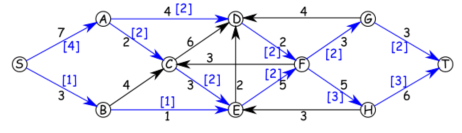
\includegraphics[width=.8\textwidth]{img/7_A1}
\end{figure}
Ogólne Jardan pomylił się - TO NIE JEST PRZEPŁYW - do $F$ ",,wpływa'' $4$ a ,,wypływa'' $5$.

\begin{figure}[H]
\centering
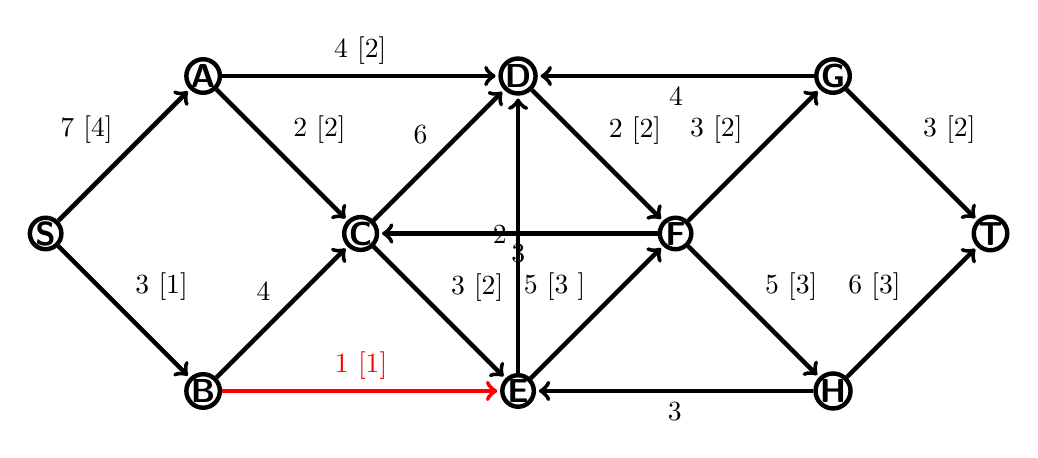
\begin{tikzpicture}[shorten >=1pt, auto, node distance=3cm, ultra thick,main node/.style={circle,draw,minimum size=.4cm,inner sep=0pt}]
\begin{scope}[every node/.style={font=\sffamily\large\bfseries}]
\node[main node] (v1) at (0,0) {S};
\node[main node] (v2) at (2,2) {A};
\node[main node] (v3) at (2,-2) {B};
\node[main node] (v4) at (4,0) {C};
\node[main node] (v5) at (6,2) {D};
\node[main node] (v6) at (6,-2) {E};
\node[main node] (v7) at (8,0) {F};
\node[main node] (v8) at (10,2) {G};
\node[main node] (v9) at (10,-2) {H};
\node[main node] (v10) at (12,0) {T};
\end{scope}
%\begin{scope}[every edge/.style={draw=black,ultra thick}]
\draw [->] (v1) edge node{3 [1]} (v3);
\draw [->] (v1) edge node{7 [4]} (v2);
\draw [->] (v2) edge node{2 [2]} (v4);
\draw [->] (v3) edge node{4} (v4);
\draw [->] (v2) edge node{4 [2]} (v5);
\draw [->] (v4) edge node{6} (v5);
\draw [->] (v4) edge node{3 [2]} (v6);
\draw [->,color=red] (v3) edge node{1 [1]} (v6);
\draw [->] (v5) edge node{2 [2]} (v7);
\draw [->] (v8) edge node{4} (v5);
\draw [->] (v6) edge node{2} (v5);
\draw [->] (v7) edge node{3} (v4);
\draw [->] (v6) edge node{5 [3
]} (v7);
\draw [->] (v7) edge node{3 [2]} (v8);
\draw [->] (v7) edge node{5 [3]} (v9);
\draw [->] (v9) edge node{3} (v6);
\draw [->] (v9) edge node{6 [3]} (v10);
\draw [->] (v8) edge node{3 [2]} (v10);
%\end{scope}
\end{tikzpicture}
\caption*{Poprawiony przepływ Jardana}
\end{figure}

\begin{figure}[H]
\centering
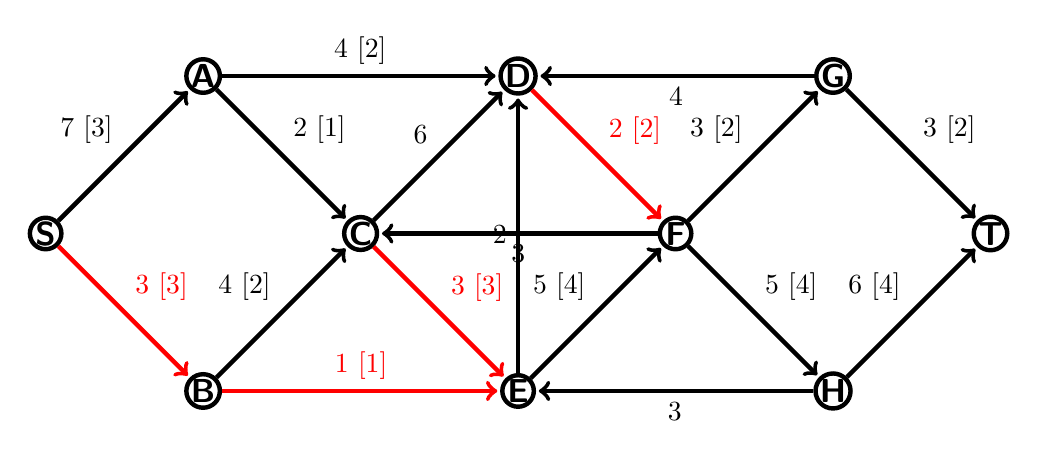
\begin{tikzpicture}[shorten >=1pt, auto, node distance=3cm, ultra thick,main node/.style={circle,draw,minimum size=.4cm,inner sep=0pt}]
\begin{scope}[every node/.style={font=\sffamily\large\bfseries}]
\node[main node] (v1) at (0,0) {S};
\node[main node] (v2) at (2,2) {A};
\node[main node] (v3) at (2,-2) {B};
\node[main node] (v4) at (4,0) {C};
\node[main node] (v5) at (6,2) {D};
\node[main node] (v6) at (6,-2) {E};
\node[main node] (v7) at (8,0) {F};
\node[main node] (v8) at (10,2) {G};
\node[main node] (v9) at (10,-2) {H};
\node[main node] (v10) at (12,0) {T};
\end{scope}
%\begin{scope}[every edge/.style={draw=black,ultra thick}]
\draw [->,color=red] (v1) edge node{3 [3]} (v3);
\draw [->] (v1) edge node{7 [3]} (v2);
\draw [->] (v2) edge node{2 [1]} (v4);
\draw [->] (v3) edge node{4 [2]} (v4);
\draw [->] (v2) edge node{4 [2]} (v5);
\draw [->] (v4) edge node{6} (v5);
\draw [->,color=red] (v4) edge node{3 [3]} (v6);
\draw [->,color=red] (v3) edge node{1 [1]} (v6);
\draw [->,color=red] (v5) edge node{2 [2]} (v7);
\draw [->] (v8) edge node{4} (v5);
\draw [->] (v6) edge node{2} (v5);
\draw [->] (v7) edge node{3} (v4);
\draw [->] (v6) edge node{5 [4]} (v7);
\draw [->] (v7) edge node{3 [2]} (v8);
\draw [->] (v7) edge node{5 [4]} (v9);
\draw [->] (v9) edge node{3} (v6);
\draw [->] (v9) edge node{6 [4]} (v10);
\draw [->] (v8) edge node{3 [2]} (v10);
%\end{scope}
\end{tikzpicture}
\caption*{Mój przepływ}
\end{figure}
Poprawiony przepływ Jardana nie największy, mój rysunek taki przepływ przedstawia. Cięcie następuje na krawędziach: $\{B;E\},\{C;E\},\{D;F\}$
\begin{align*}
Z=\{T,G,F,E,H\}\\
B=\{S,A,B,C,D\}\\
\mathsf{val}(f)=1+3+2=6\\
\mathsf{cap}(B,Z)=6
\end{align*}

\paragraph{A2}
\begin{enumerate}[label=\alph*)]
\begin{figure}[H]
\centering
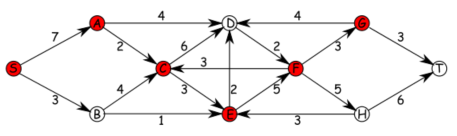
\includegraphics[width=.8\textwidth]{img/7_A2}
\end{figure}
\item Oblicz pojemność cięcia wyznaczonego przez podany podział (X,Y ), gdzie X to zbiór wierzchołków czerwonych, a Y – zbiór pozostałych wierzchołków sieci.

\begin{definition}
Pojemnością cięcia $(S, \bar{S})$, oznaczaną jako $\mathsf{cap}(S, \bar{S})$, nazywamy sumę pojemności strzałek wychodzących z $S$, tzn. strzałek o początku w $S$ i końcu w $\bar{S}$.
\end{definition}
\begin{align*}
&X=\{S,A,C,E,F,G\}\\
&Y=\{B,D,H,T\}\\
&\mathsf{cap}(X,Y)=\mathsf{cap}(S,B)+\mathsf{cap}(A,D)+\mathsf{cap}(C,D)+\mathsf{cap}(E,D)+\mathsf{cap}(F,H)+\mathsf{cap}(G,T)\\
&\mathsf{cap}(X,Y)=3+4+6+2+5+3=23
\end{align*}
\item Czy (X,Y ) jest najmniejszym Cięciem? Jeśli tak, to uzasadnij; Jeśli nie – wskaż lepszy podział.

\textbf{Nie, nie jest, }
\begin{align*}
X=\{S,A,B,C,D,E\}\\
Y=\{F,G,H,T\}\\
\mathsf{cap}(X,Y)=2+5=7
\end{align*}
\begin{figure}[H]
\centering
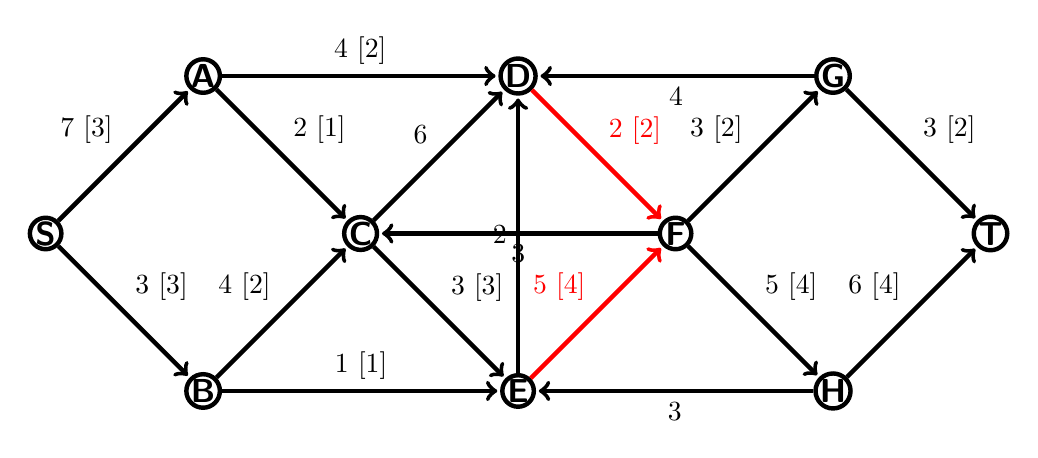
\begin{tikzpicture}[shorten >=1pt, auto, node distance=3cm, ultra thick,main node/.style={circle,draw,minimum size=.4cm,inner sep=0pt}]
\begin{scope}[every node/.style={font=\sffamily\large\bfseries}]
\node[main node] (v1) at (0,0) {S};
\node[main node] (v2) at (2,2) {A};
\node[main node] (v3) at (2,-2) {B};
\node[main node] (v4) at (4,0) {C};
\node[main node] (v5) at (6,2) {D};
\node[main node] (v6) at (6,-2) {E};
\node[main node] (v7) at (8,0) {F};
\node[main node] (v8) at (10,2) {G};
\node[main node] (v9) at (10,-2) {H};
\node[main node] (v10) at (12,0) {T};
\end{scope}
%\begin{scope}[every edge/.style={draw=black,ultra thick}]
\draw [->] (v1) edge node{3 [3]} (v3);
\draw [->] (v1) edge node{7 [3]} (v2);
\draw [->] (v2) edge node{2 [1]} (v4);
\draw [->] (v3) edge node{4 [2]} (v4);
\draw [->] (v2) edge node{4 [2]} (v5);
\draw [->] (v4) edge node{6} (v5);
\draw [->] (v4) edge node{3 [3]} (v6);
\draw [->] (v3) edge node{1 [1]} (v6);
\draw [->,color=red] (v5) edge node{2 [2]} (v7);
\draw [->] (v8) edge node{4} (v5);
\draw [->] (v6) edge node{2} (v5);
\draw [->] (v7) edge node{3} (v4);
\draw [->,color=red] (v6) edge node{5 [4]} (v7);
\draw [->] (v7) edge node{3 [2]} (v8);
\draw [->] (v7) edge node{5 [4]} (v9);
\draw [->] (v9) edge node{3} (v6);
\draw [->] (v9) edge node{6 [4]} (v10);
\draw [->] (v8) edge node{3 [2]} (v10);
%\end{scope}
\end{tikzpicture}
\caption*{Mój przepływ}
\end{figure}
\end{enumerate}


\paragraph{A3} Rozważmy pewną sieć.
$$\mathsf{cap}(X,Y)\geq \mathsf{MINCUT}=\mathsf{MAXFLOW}\geq \mathsf{val}(f)$$
\begin{enumerate}[label=\alph*)]
\item Załóżmy, że w sieci istnieje pewne Cięcie o pojemności 10. Jakie wynika z tego oszacowanie ma
wartość największego przypływu?

$\mathsf{cap}(S,\bar{S})=10$ $\Rightarrow$ $\mathsf{MAXFLOW}\leq 10$?
\item Załóżmy, że w sieci istnieje pewien przepływ o wartości 8. Jakie wynika z tego oszacowanie ma pojemność najmniejszego cięcia?

$\mathsf{val}(f)=8$ $\Rightarrow$ $\Rightarrow$ $\mathsf{MINCUT}\geq 8$?
\end{enumerate}

\paragraph{A4} Najmniejsze Cięcie w pewnej sieci jest wyznaczone przez trzy strzałki: (a,b) o pojemności 3, (c,d) o
pojemności 4 i (a,d) o pojemności 2, przy czym wierzchołki a, c leżą po stronie źródła, a wierzchołki b i d
po stronie ujścia.
\begin{figure}[H]
\centering
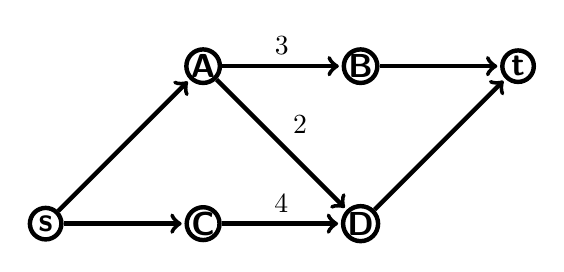
\begin{tikzpicture}[shorten >=1pt, auto, node distance=3cm, ultra thick,main node/.style={circle,draw,minimum size=.4cm,inner sep=0pt}]
\begin{scope}[every node/.style={font=\sffamily\large\bfseries}]
\node[main node] (v0) at (0,0) {s};
\node[main node] (v1) at (2,2) {A};
\node[main node] (v3) at (2,0) {C};
\node[main node] (v2) at (4,2) {B};
\node[main node] (v4) at (4,0) {D};
\node[main node] (v5) at (6,2) {t};
\end{scope}
%\begin{scope}[every edge/.style={draw=black,ultra thick}]
\draw [->] (v0) edge (v1);
\draw [->] (v0) edge (v3);
\draw [->] (v1) edge node{3} (v2);
\draw [->] (v1) edge node{2} (v4);
\draw [->] (v3) edge node{4} (v4);
\draw [->] (v2) edge (v5);
\draw [->] (v4) edge (v5);

%\end{scope}
\end{tikzpicture}
\caption*{\#rysunek}
\end{figure}
\begin{enumerate}[label=\alph*)]
\item Ile wynosi największy przepływ w tej sieci?

$\mathsf{val}(f)=\mathsf{val}(A,B)+\mathsf{val}(A,D)+\mathsf{val}(C,D)=3+2+4=9$
\item Czy Jeśli zwiększymy o jeden pojemności każdej ze strzałek (a,b), (c,d) i (a,d) o 1, to wartość największego przepływu na pewno się zwiększy? Jeżeli tak, to uzasadnij dlaczego; jeżeli nie, to podaj kontrprzykład.

\textbf{NIE} nie znamy pojemności $\{(s,A),(s,C),(B,t),(D,t),\}$
\end{enumerate}


\paragraph{A5} Dana jest sieć D, w której każda krawędź z ma pojemność jeden. Załóżmy, że w sieci tej istnieje k
(k > 1) krawędziowo rozłącznych ścieżek skierowanych ze źródła do ujścia. Uzasadnij, że:
\begin{enumerate}[label=\alph*)]
\item wartość największego przepływu w D wynosi co najmniej k.

Mamy $k$-rozłącznych ścieżek (nie mają części wspólnych), czyli możemy znaleźć $k$ strzałek. Mamy podane, że istnieje k ścieżek, co oznacza, że wierzchołki są zbilansowane - może być więcej niż $k$ strzałek.

\textit{Wytłumaczenie z ,,przymrożeniem oka''}
Jeżeli w sieci $D$ istnieje $k$ rozłącznych ścieżek (rozłączne, czyli nie mają nic wspólne) to przepływ sieci ma wartość $\mathsf{val}(f)=\sum _1^k 1 = k$
\item pojemność każdego cięcia w D wynosi przynajmniej k.

Wynika z a) + wzór: $\mathsf{cap}(X,Y)\geq \mathsf{MINCUT}=\mathsf{MAXFLOW}\geq \mathsf{val}(f)$
\end{enumerate}

\paragraph{A6} Oceń poprawność każdego z poniższych zdań. W każdym przypadku poprzyj odpowiedź, w zależności
od potrzeby, uzasadnieniem ogólnym, przykładem lub kontrprzykładem. poprawność przykładów/kontr przykładów też należy uzasadnić.
\begin{enumerate}[label=\alph*)]
\item Jeżeli w sieci istnieje Cięcie o pojemności 3, to największy przepływ w tej sieci ma wartość 3.

\textbf{NIE} wzór: $\mathsf{cap}(X,Y)\geq \mathsf{MINCUT}=\mathsf{MAXFLOW}\geq \mathsf{val}(f)$
\begin{figure}[H]
\centering
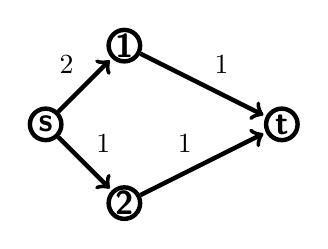
\begin{tikzpicture}[shorten >=1pt, auto, node distance=3cm, ultra thick,main node/.style={circle,draw,minimum size=.4cm,inner sep=0pt}]
\begin{scope}[every node/.style={font=\sffamily\large\bfseries}]
\node [main node](v0) at (0,0) {s};
\node [main node](v1) at (1,1) {1};
\node [main node](v2) at (1,-1) {2};
\node [main node](v3) at (3,0) {t};
\end{scope}
\draw [->] (v0) edge node {2} (v1);
\draw [->] (v0) edge node {1} (v2);
\draw [->] (v1) edge node {1} (v3);
\draw [->] (v2) edge node {1} (v3);
\end{tikzpicture}
\end{figure} 
\item Jeżeli w sieci istnieje przepływ o wartości 2, to najmniejsze Cięcie w tej sieci ma pojemność 2.

\textbf{NIE}
\begin{figure}[H]
\centering
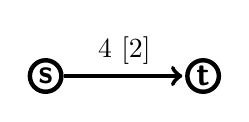
\begin{tikzpicture}[shorten >=1pt, auto, node distance=3cm, ultra thick,main node/.style={circle,draw,minimum size=.4cm,inner sep=0pt}]
\begin{scope}[every node/.style={font=\sffamily\large\bfseries}]
\node [main node](v0) at (0,0) {s};
\node [main node](v1) at (2,0) {t};
\end{scope}
\draw [->] (v0) edge node {4 [2]} (v1);
\end{tikzpicture}
\end{figure} 
przepływ ma wartość $2$ ale cięcie ma wartość $4$
\item Jeśli w sieci zmniejszymy pojemność każdej strzałki, to zmniejszy się pojemność najmniejszego cięcia.

\textbf{NIE} jak i \textbf{TAK}
\begin{multicols}{2}
\textbf{NIE}
\begin{figure}[H]
\centering
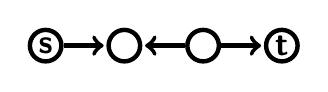
\begin{tikzpicture}[shorten >=1pt, auto, node distance=3cm, ultra thick,main node/.style={circle,draw,minimum size=.4cm,inner sep=0pt}]
\begin{scope}[every node/.style={font=\sffamily\large\bfseries}]
\node [main node](v0) at (0,0) {s};
\node [main node](v1) at (1,0) {};
\node [main node](v2) at (2,0) {};
\node [main node](v3) at (3,0) {t};
\end{scope}
\draw [->] (v0) edge (v1);
\draw [->] (v2) edge (v1);
\draw [->] (v2) edge (v3);
\end{tikzpicture}
\end{figure} 
\vfill\null
\columnbreak
\textbf{TAK}
\begin{figure}[H]
\centering
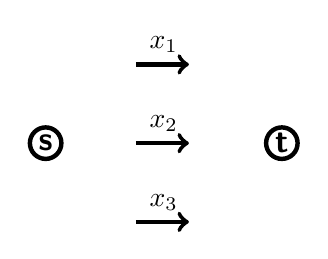
\begin{tikzpicture}[shorten >=1pt, auto, node distance=3cm, ultra thick,main node/.style={circle,draw,minimum size=.4cm,inner sep=0pt}]
\begin{scope}[every node/.style={font=\sffamily\large\bfseries}]
\node [main node] at (0,0) {s};
\node (v11) at (1,0) {};
\node (v12) at (2,0) {};
\node (v21) at (1,1) {};
\node (v22) at (2,1) {};
\node (v31) at (1,-1) {};
\node (v32) at (2,-1) {};
\node [main node] at (3,0) {t};
\end{scope}
\draw [->] (v11) edge node {$x_2$} (v12);
\draw [->] (v21) edge node {$x_1$} (v22);
\draw [->] (v31) edge node {$x_3$} (v32);
\end{tikzpicture}
\end{figure} 
$\mathsf{cut}=\sum ^nx$
\begin{figure}[H]
\centering
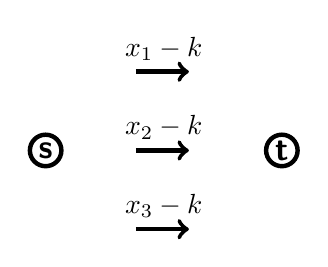
\begin{tikzpicture}[shorten >=1pt, auto, node distance=3cm, ultra thick,main node/.style={circle,draw,minimum size=.4cm,inner sep=0pt}]
\begin{scope}[every node/.style={font=\sffamily\large\bfseries}]
\node [main node] at (0,0) {s};
\node (v11) at (1,0) {};
\node (v12) at (2,0) {};
\node (v21) at (1,1) {};
\node (v22) at (2,1) {};
\node (v31) at (1,-1) {};
\node (v32) at (2,-1) {};
\node [main node] at (3,0) {t};
\end{scope}
\draw [->] (v11) edge node {$x_2-k$} (v12);
\draw [->] (v21) edge node {$x_1-k$} (v22);
\draw [->] (v31) edge node {$x_3-k$} (v32);
\end{tikzpicture}
\end{figure} 
$\mathsf{cut}=\sum ^nx-nk$\\
I to zachodzi dla każdego $k$
\end{multicols}

\item Jeśli w sieci zwiększymy pojemność każdej strzałki wychodzącej ze źródła, to zwiększy się wartość największego przepływu.

\textbf{NIE}: A co ze strzałkami do ujścia?
\item Istnieje sieć, w której są co najmniej dwa różne największe przepływy.

\textbf{TAK}
\begin{figure}[H]
\centering
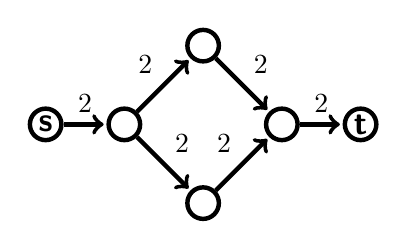
\begin{tikzpicture}[shorten >=1pt, auto, node distance=3cm, ultra thick,main node/.style={circle,draw,minimum size=.4cm,inner sep=0pt}]
\begin{scope}[every node/.style={font=\sffamily\large\bfseries}]
\node [main node](v0) at (0,0) {s};
\node [main node](v1) at (1,0) {};
\node [main node](v2) at (2,1) {};
\node [main node](v3) at (2,-1) {};
\node [main node](v4) at (3,0) {};
\node [main node](v5) at (4,0) {t};
\end{scope}
\draw [->] (v0) edge node{2} (v1);
\draw [->] (v1) edge node{2} (v2);
\draw [->] (v1) edge node{2} (v3);
\draw [->] (v2) edge node{2} (v4);
\draw [->] (v3) edge node{2} (v4);
\draw [->] (v4) edge node{2} (v5);
\end{tikzpicture}
\end{figure}
\item Istnieje sieć, w której są co najmniej dwa różne najmniejsze cięcia.

\textbf{TAK}
\begin{figure}[H]
\centering
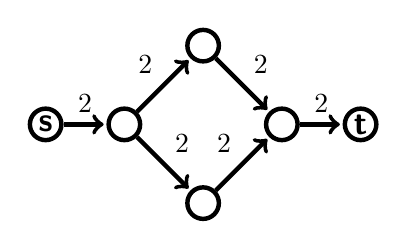
\begin{tikzpicture}[shorten >=1pt, auto, node distance=3cm, ultra thick,main node/.style={circle,draw,minimum size=.4cm,inner sep=0pt}]
\begin{scope}[every node/.style={font=\sffamily\large\bfseries}]
\node [main node](v0) at (0,0) {s};
\node [main node](v1) at (1,0) {};
\node [main node](v2) at (2,1) {};
\node [main node](v3) at (2,-1) {};
\node [main node](v4) at (3,0) {};
\node [main node](v5) at (4,0) {t};
\end{scope}
\draw [->] (v0) edge node{2} (v1);
\draw [->] (v1) edge node{2} (v2);
\draw [->] (v1) edge node{2} (v3);
\draw [->] (v2) edge node{2} (v4);
\draw [->] (v3) edge node{2} (v4);
\draw [->] (v4) edge node{2} (v5);
\end{tikzpicture}
\end{figure}
\item Jeżeli w sieci są co najmniej dwa różne największe przepływy, to w sieci tej istnieją przynajmniej dwa różne najmniejsze cięcia.

\textbf{NIE}
\begin{figure}[H]
\centering
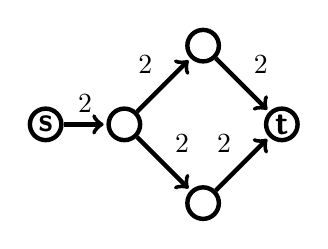
\begin{tikzpicture}[shorten >=1pt, auto, node distance=3cm, ultra thick,main node/.style={circle,draw,minimum size=.4cm,inner sep=0pt}]
\begin{scope}[every node/.style={font=\sffamily\large\bfseries}]
\node [main node](v0) at (0,0) {s};
\node [main node](v1) at (1,0) {};
\node [main node](v2) at (2,1) {};
\node [main node](v3) at (2,-1) {};
\node [main node](v4) at (3,0) {t};
\end{scope}
\draw [->] (v0) edge node{2} (v1);
\draw [->] (v1) edge node{2} (v2);
\draw [->] (v1) edge node{2} (v3);
\draw [->] (v2) edge node{2} (v4);
\draw [->] (v3) edge node{2} (v4);
\end{tikzpicture}
\end{figure}
\item Jeśli w sieci istnieją przynajmniej dwa różne najmniejsze cięcia, to w tej sieci istnieją co najmniej dwa różne największe przepływy.

\textbf{NIE}
\begin{figure}[H]
\centering
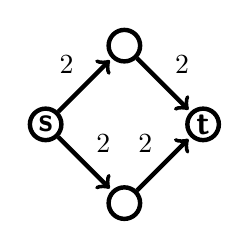
\begin{tikzpicture}[shorten >=1pt, auto, node distance=3cm, ultra thick,main node/.style={circle,draw,minimum size=.4cm,inner sep=0pt}]
\begin{scope}[every node/.style={font=\sffamily\large\bfseries}]
\node [main node](v1) at (1,0) {s};
\node [main node](v2) at (2,1) {};
\node [main node](v3) at (2,-1) {};
\node [main node](v4) at (3,0) {t};
\end{scope}

\draw [->] (v1) edge node{2} (v2);
\draw [->] (v1) edge node{2} (v3);
\draw [->] (v2) edge node{2} (v4);
\draw [->] (v3) edge node{2} (v4);
\end{tikzpicture}
\end{figure}
\item Jeżeli wszystkie pojemności strzałek w sieci są  całkowite, to wszystkie największe przepływy przypisują wszystkim strzałkom całkowite wartości.

\textbf{NIE}
\begin{figure}[H]
\centering
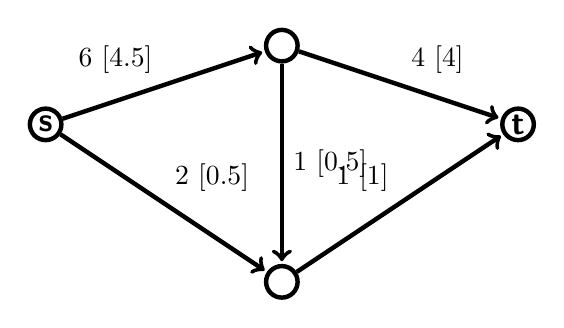
\begin{tikzpicture}[shorten >=1pt, auto, node distance=3cm, ultra thick,main node/.style={circle,draw,minimum size=.4cm,inner sep=0pt}]
\begin{scope}[every node/.style={font=\sffamily\large\bfseries}]
\node [main node](v1) at (-1,0) {s};
\node [main node](v2) at (2,1) {};
\node [main node](v3) at (2,-2) {};
\node [main node](v4) at (5,0) {t};
\end{scope}

\draw [->] (v1) edge node{6 [4.5]} (v2);
\draw [->] (v1) edge node{2 [0.5]} (v3);
\draw [->] (v2) edge node{4 [4]} (v4);
\draw [->] (v2) edge node{1 [0.5]} (v3);
\draw [->] (v3) edge node{1 [1]} (v4);
\end{tikzpicture}
\end{figure}
\end{enumerate}

\subsection{Zadania domowe B}
\paragraph{B1} Fabryka czekolady produkuje 50 różnych smakołyków. Fabryka chce zbadać kwestionariuszami opinie 100 klientów o swoich produktach. Oto założenia, jakie kwestionariusze muszą
spełniać:
\begin{itemize}
\item Nie można pytać o produkt, którego klient nigdy nie kupił.
\item każdy klient jest pytany o co najwyżej 10 produktów.
\item każdy produkt musi być oceniony przez dokładnie 5 klientów
\end{itemize}
Naszym celem jest rozstrzygnąć, czy można wg tych zasad kwestionariusze ułożyć.
\begin{enumerate}[label=\alph*)]
\item Zaprojektuj tradycyjną sieć D z jednym ujściem i źródłem tak, by problem ułożenia kwestionariuszy
sprowadzić do równoważnego mu problemu badania przepływu w sieci D.
\item Jaki warunek musi spełniać przepływ w sieci D, aby ułożenie kwestionariuszy było możliwe?
\item Jak na podstawie przepływu w sieci D zbudować kwestionariusze?
\end{enumerate}

\paragraph{B2} Rozwiąż zadanie analogiczne do poprzedniego, zastępując warunek ,,dokładnie 5 klientów'' przez ,,przynajmniej 5 klientów''.

\paragraph{B3} Chcemy zbadać kwestionariuszami opinie klientów X, Y , Z, U, W o produktach A, B, C, D, E. Na rysunku po lewej stronie zaznaczono krawędziami, który klient kupi l które produkty. Oto założenia, jakie kwestionariusze muszą spełniać:
\begin{itemize}
\item Nie można pytać o produkt, którego klient nigdy nie kupił.
\item każdy klient i jest pytany o co najwyżej k i produktów, dla i = X,Y,Z,U,W.
\item każdy produkt musi być oceniony przez dokładnie 2 klientów.
\end{itemize}
Aby rozstrzygnąć, czy można wg tych zasad kwestionariusze ułożyć, zbudowaliśmy sieć S 2 przedstawioną po prawej stronie. Jaki warunek musi być spełniony dla sieci $S_2$ , aby ułożenie kwestionariuszy było możliwe? odpowiedź należy (oczywiście) dokładnie uzasadnić.
\begin{figure}[H]
\centering
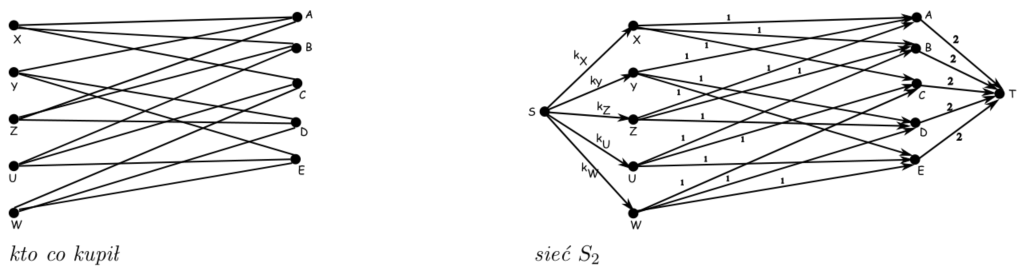
\includegraphics[width=.9\textwidth]{img/7_B3}
\end{figure}

\paragraph{B4} Dane są liczby $k_i\in \{0,1,2,3\}$ oraz $r_j\in \{0,1,2,3\}$, dla $i = X,Y,Z,U,W$ oraz $j = A,B,C,D,E$. Pięciu krasnoludków $X, Y , Z, U, W$, chce rozesłać prezenty do rodzin $A, B, C, D, E$ wg następujących zasad:
\begin{enumerate}[label=\alph*)]
\item Krasnoludek $i$ musi wysłać dokładnie $k_i$ prezentów, dla $i = X,Y,Z,U,W$.
\item Rodzina $j$ musi dostać dokładnie $r_j$ prezentów, dla $j = A,B,C,D,E$.
\item każdy krasnoludek może wysłać każdej z rodzin co najwyżej jeden prezent.
\item Na rysunku po lewej stronie zaznaczono krawędziami, który krasnoludek której rodzinie może wysłać prezent.
\end{enumerate}
Załóżmy, że takie rozesłanie prezentów jest możliwe i wiadomo, jak krasnoludki powinny rozesłać prezenty. Czy wynika z tego, że w sieci $S_2$ po prawej istnieje przepływ o wartości $$r_A + r_B + r_C + r_D + r_E\ ?$$ Jeśli nie, to uzasadnij dlaczego; Jeśli tak, to opisz ten przepływ.
\begin{figure}[H]
\centering
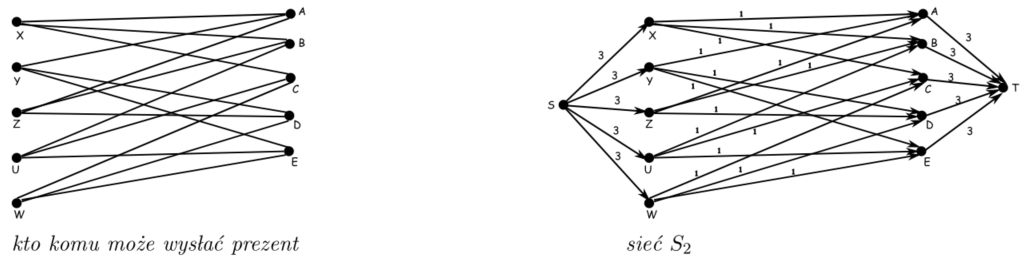
\includegraphics[width=.9\textwidth]{img/7_B4}
\end{figure}

Uwaga: Liczby $k_i \in \{0, 1, 2, 3\}$ oraz $r_j \in \{0, 1, 2, 3\}$ są dowolne i nie muszą być równe $3$.

\paragraph{B5} Rozważmy poniższą korespondencyjną  sieć H hobbistów, wysyłających sobie kartki z pozdrowieniami. Każdemu człowiekowi (wierzchołkowi) przypisano liczbę całkowitą, która mówi, jaka musi być różnica między liczbą  kartek przez niego otrzymanych i wysłanych. Innymi słowy, ujemne zapotrzebowanie wierzchołka oznacza, że hobbista ma więcej kartek wysłać niż dostać, a dodatnie – że więcej kartek powinien dostać niż wysłać. krawędziom między hobbistami przypisano nieujemne liczby całkowite, z których – jak widać – tylko niektóre są nam znane. Pojedyncza liczba przypisana krawędzi (i,j) ogranicza z góry liczbę kartek, jakie hobbista i może wysłać hobbiście j. Jeżeli krawędzi przypisano dwie liczby, to są one ograniczeniami odpowiednio dolnymi i górnymi na dopuszczalną liczbę wysłanych kartek. Mówimy, że H może w rzeczywistości zadziałał, jeżeli ludzie mogą wysłać i dostać kartki zgodnie ze swoimi zapotrzebowaniem (i wymaganiami na krawędziach). Ustalmy sieć hobbistów H taką jak na rysunku H. Obok widzimy standardową sieć D ze źródłem S i ujściem T.
\begin{enumerate}[label=\alph*]
\item Załóżmy, że korespondencyjna sieć H może w rzeczywistości zadziałał. Co na tej podstawie można powiedzieć o największym przepływie w sieci D?
\item Załóżmy, że wartość największego przepływu w sieci D wynosi 5. Co możemy powiedzieć na temat możliwości zadziałania sieci hobbistów H?
\end{enumerate}
\begin{figure}[H]
\centering
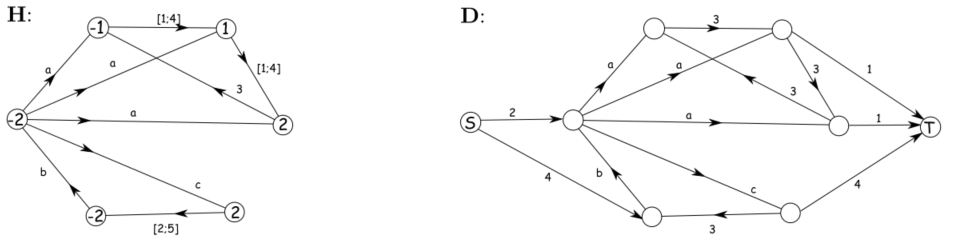
\includegraphics[width=.9\textwidth]{img/7_B5}
\end{figure}

\paragraph{B6} Rozważmy świąteczną sieć ludzi robiących sobie prezenty. Każdemu przypisujemy liczbę, która mówi, jaka musi być różnica między liczbą prezentów przez niego otrzymanych i wysłanych. krawędziom skierowanym między ludźmi i oraz j przypisujemy przepustowości określone przedziałami [d ij ,g ij ], co oznacza, że i musi wysłać j co najmniej d ij prezentów, ale nie więcej niż g ij . Jak rozstrzygnąć, czy taka sieć może w rzeczywistości zadziałał? Zakładamy (jak zwykle), że można tu korzystać z gotowego algo rytmu, znajdującego największy przepływ i najmniejsze cięcie w standardowych sieciach z jednym źródłem i jednym ujściem.

\paragraph{B7} Jak za pomocą algorytmu wyznaczającego największy przepływ wyznaczyć największe skojarzenie w grafie dwudzielnym?

\paragraph{B8 * } Jesteś szefem firmy informatycznej i rozważasz rozpoczęcie kilku projektów. między projektami są pewne zależności, tzn. wdrożenie jednego wymaga być może wdrożenia najpierw kilku innych. Wykonanie danego projektu oznacza albo niezerowe koszty, albo niezerowe zyski, przy czym wykonanie czegoś kosztownego może umożliwić wdrożenie czegoś niezwykle zyskownego. Możesz zdecydować, że firma wykona tylko część projektów, ale oczywiście nie można zdecydować, że zajmie się tylko projektami ze zbioru A, Jeśli jakiś projekt konieczny do ich wykonania jest z A wyłączony. Zakładamy, że spełnione są następujące warunki.
\begin{itemize}
\item Projekt nie może generować jednocześnie zysku i kosztów. Jeśli generuje zysk, nazywamy go zyskownym, a Jeśli generuje koszt, to nazywamy go kosztownym.
\item Jeśli projekt x jest konieczny do wykonania projektu y, to x jest kosztowny, a y zyskowny.
\end{itemize}
Twoim zadaniem jest wybrać jak najlepiej zbiór projektów do realizacji, znając powiązania między projektami, przewidywane profity i koszty generowane przez każdy projekt z osobna. Celem jest jak najlepszy wynik finansowy po zakończeniu wszystkich projektów. Zaprojektuj algorytm, bazując na gotowym algorytmie znajdującym największy przepływ i najmniejsze Cięcie w standardowych sieciach z jednym źródłem i jednym ujściem.


\subsection{Zadania}
Zakładamy, że we wszystkich zadaniach można korzystać z gotowego algorytmu, znajdującego największy przepływ (i najmniejsze Cięcie) w standardowych sieciach z jednym źródłem i jednym ujściem.

\paragraph{Zad.1} Cztery kury zniosły jaja. i-ta kura zniosła i jaj. Kury chcą wysłać wszystkie jaja do 5 rodzin, korzystając z sieci 3 pośredników. każda rodzina musi dostać po 2 jaja. Na rysunku podane są przepustowości łączy, czyli liczby jaj, jakie mogą być przesłane bezpośrednio między dwoma węzłami naszej wielkanocnej sieci (tworzonej przez kury, pośredników i rodziny). 
\begin{itemize}
\item Sprawdź w domu, która z podanych sieci wielkanocnych zadziała, tzn. w której sieci jaja mogą być rozesłane zgodnie z powyższymi zasadami. W tym przypadku opisz, kto komu ile jaj wysyła.
\item Przetłumacz problem rozesłania jaj w pierwszej sieci na równoważny mu problem przepływu w standardowej sieci z jednym źródłem i jednym ujściem. Jaki warunek jest konieczny i dostateczny, by sieć prezentowa mogła zadziałał?
\item Rozważmy dowolną sieć wielkanocną, tzn. z dowolną liczbą kur, pośredników i rodzin, pojemnościami krawędzi i wymaganiami związanymi z tym, ile jaj dana kura zniosła oraz ile jaj dana rodzina potrzebuje. Przetłumacz problem na równoważny mu problem przepływu w standardowych sieciach z jednym źródłem i jednym ujściem. Jaki warunek jest konieczny i dostateczny, by sieć wielkanocna mogła zadziałał?
\end{itemize}
\begin{figure}
\centering
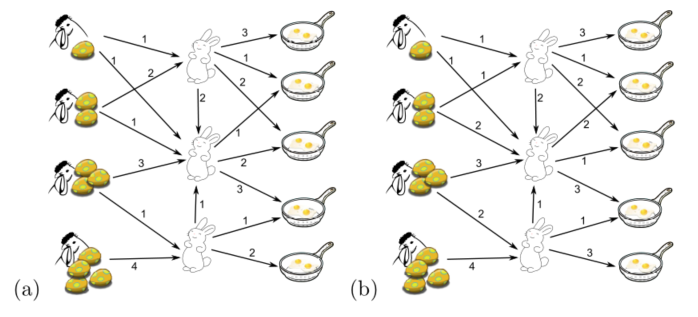
\includegraphics[width=.8\textwidth]{img/7_Z1}
\end{figure}


\paragraph{Zad.2} Rozważmy korespondencyjną sieć hobbistów, wysyłających sobie kartki z pozdrowieniami. Każdemu człowiekowi i przypisujemy liczbę całkowitą $i$ , która mówi, jaka musi być różnica między liczbą kartek przez niego otrzymanych i wysłanych. krawędziom skierowanym między ludźmi $i$ oraz $j$ przypisujemy nieujemne liczby całkowite $k_{ij}$ , co oznacza, że $i$ może wysłać $j$ co najwyżej $k_{ij}$ kartek.\\
Jak rozstrzygnąć, czy opisana korespondencyjna sieć może w rzeczywistości zadziałał, tzn. czy ludzie mogą wysłać i dostać kartki zgodnie ze swoimi zapotrzebowania mi? Jak powinni wysyłać kartki?

\paragraph{Zad.3} Mamy do rozwiązania następujący problem optymalizacyjny. W mieście ukrywają się przestępcy. Policja zna prawdopodobne miejsca kryjówek przestępców. Przestępcy mogą odpuścić miasto jedynie kilkoma wyjazdami, również policji znanymi. Dla każdej ulicy wiadomo, ilu policjantów potrzeba, by ją zablokować. Zadaniem policji jest przeprowadzić skuteczną blokadę ulic przy pomocy jak najmniejszej liczby policjantów. Dla jasności obrazu podajemy przykładową mapkę miasta. K1,K2 to miejsca, w których mogą ukrywać się przestępcy, a W,N,E,S – wyjazdy z miasta. Liczby przy ulicach określają, ilu policjantów potrzeba, by zablokować ulicę. Ulice są dwukierunkowe. Zaproponuj algorytm rozwiązujący problem dla dowolnego miasta i przedstaw jego działanie na podanej mapce. Dane wejściowe to plan miasta z zaznaczonymi potencjalnymi kryjówkami przestępców, możliwymi miejscami wyjazdu z miasta i liczbą policjantów konieczną do zablokowania każdej ulicy. Algorytm powinien zwracać optymalną liczbę policjantów i ich rozmieszczenie na ulicach.
\begin{figure}
\centering
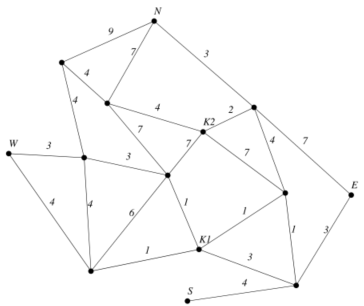
\includegraphics[width=.8\textwidth]{img/7_Z3}
\end{figure}

\paragraph{Zad.4} Na pewnym kameralnym uniwersytecie wykłady prowadzi czterech profesorów, a ćwiczenia – dziewięciu adiunktów. Przedmiotów jest dużo, zajęcia z każdego przedmiotu trwają, jak to zwykle bywa,
przez cały semestr. Profesorowie powinni hospitować ćwiczenia do prowadzonych przez siebie wykładów.
Przy tym następujące warunki muszą być spełnione:
\begin{itemize}
\item każdy profesor musi w semestrze przeprowadzić dokładnie 4 hospitacje.
\item Profesor może hospitować tylko ćwiczenia do prowadzonych przez siebie wykładów.
\item każdy profesor może hospitować zajęcia prowadzone przez danego adiunkta co najwyżej dwukrotnie.
\item każdy adiunkt może mieć na wszystkich swoich zajęciach w czasie semestru co najwyżej 6 hospitacji.
\end{itemize}
Jak rozstrzygnąć, czy można ułożyć semestralny plan hospitacji, spełniający wszystkie powyższe warunki?

\paragraph{Zad.5} Zadanie analogiczne do zad.4, ale zamiast ,,dokładnie 4 hospitacje” są  ,,przynajmniej 4 hospitacje”.
